\documentclass{beamer}

\usetheme{metropolis}

\usepackage{xparse}
\usepackage{xfrac}
\usepackage[siunitx, american]{circuitikz}
\usepackage{hyperref}
\usepackage{cancel}
\usepackage{amssymb}
\usepackage{amsmath}
\usepackage{graphicx}
\usetikzlibrary{automata, arrows}

\makeatletter
\renewcommand*\env@matrix[1][*\c@MaxMatrixCols c]{%
  \hskip -\arraycolsep
  \let\@ifnextchar\new@ifnextchar
  \array{#1}}
\makeatother

\title{EECS 16A Midterm 1 Review Session}
\author{Presented by \textless NAMES \textgreater (HKN)}
\date{}


\begin{document}

\begin{frame}

\titlepage

\end{frame}

\begin{frame}[t]\vspace{20pt}
\frametitle{Disclaimer}
Although some of the presenters may be course staff, the material covered in the review session may not be an accurate representation of the topics covered in and difficulty of the exam.

\vspace{20pt}
Slides are posted at --- on Piazza.

\end{frame}


\begin{frame}[t]\vspace{20pt}
\frametitle{HKN Drop-In Tutoring}

\begin{itemize}
\item These details should be edited
\end{itemize}

\end{frame}

\section*{Systems of Equations and Gaussian Elimination}

\begin{frame}[t]\vspace{20pt}
\frametitle{Vectors}
Conceptually, a vector is a collection of numbers that each represent a variable. If there are $n$ variables, then the vector is $n$-dimensional.

Example: \newline
A point in 3D can be represented as $(x,y,z)$
In vector form, this would be represented as $\begin{bmatrix} x \\ y \\ z \\ \end{bmatrix}$

\end{frame}


\begin{frame}[t]\vspace{5pt}
\frametitle{Matrices}
\begin{itemize}
\item Collection of \textbf{vectors}
\item 2D table for \textbf{storing data}
	\begin{itemize}
		\item[$\circledcirc$] Systems of equations for imaging observations
	\end{itemize}
\item Notable/useful matrices
	\begin{itemize}
		\item[$\circledcirc$] Identity matrix
		\item[$\circledcirc$] Augmented matrices
		\item[$\circledcirc$] Rotation matrix
		\item[$\circledcirc$] Many others!
	\end{itemize}
\end{itemize}

Augmented:
$\begin{bmatrix}[ccc|c]
1 & -2 & 3 & 7\\
2 & 1 & 1 & 4\\
-3 & 2 & 3-2& 10\\
\end{bmatrix}$

Rotation: \hspace{9pt}
$\begin{bmatrix}
\cos{\theta} & -\sin{\theta} \\
\sin{\theta} & \cos{\theta} \\

\end{bmatrix}$

\end{frame}



\begin{frame}[t]\vspace{10pt}
\frametitle{Matrix Transformations}

Matrices are often used to perform transformations, especially 
\newline in $\mathbb{R}^2$ \newline\newline
Two important transformations:

\begin{figure}[!tbp]
  \centering
  \begin{minipage}[b]{0.3\textwidth}
    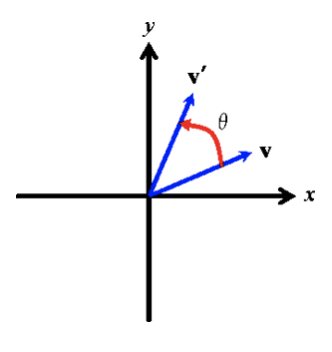
\includegraphics[width=\textwidth]{./images/rotation.png}
    \caption{Rotation}
  \end{minipage}
  \hfill
  \begin{minipage}[b]{0.3\textwidth}
    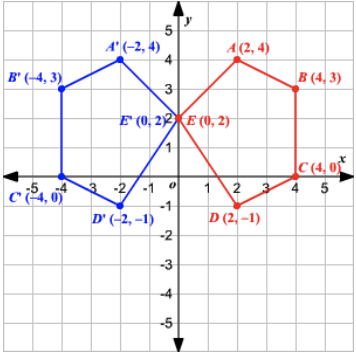
\includegraphics[width=\textwidth]{./images/reflection.png}
    \caption{Reflection}
  \end{minipage}
\end{figure}
\end{frame}


\end{document}